\documentclass{standalone}
\usepackage{etex}
\PassOptionsToPackage{rgb}{xcolor}
\usepackage{tikz}
\usepackage{pgfplots}
\usepackage{amsmath}
\usepackage{tkz-fct}
\usepackage{makecell}
\usepackage{mathrsfs}
\usepackage{pifont}
\usepackage{textcomp}
\newcommand{\xmax}{10}
\newcommand{\ymax}{10}
\usetikzlibrary{shapes.geometric,arrows,backgrounds,calc,trees,decorations.pathmorphing,patterns,3d,arrows.meta,decorations.text,}
\tikzset{>={Stealth[width=1.2mm,length=1.2mm]},box/.style={draw=none,fill=none,align=center,execute at begin node=\setlength{\baselineskip}{9pt}}}
\begin{document}
\pgfplotsset{compat=1.11,axis line style={white}}
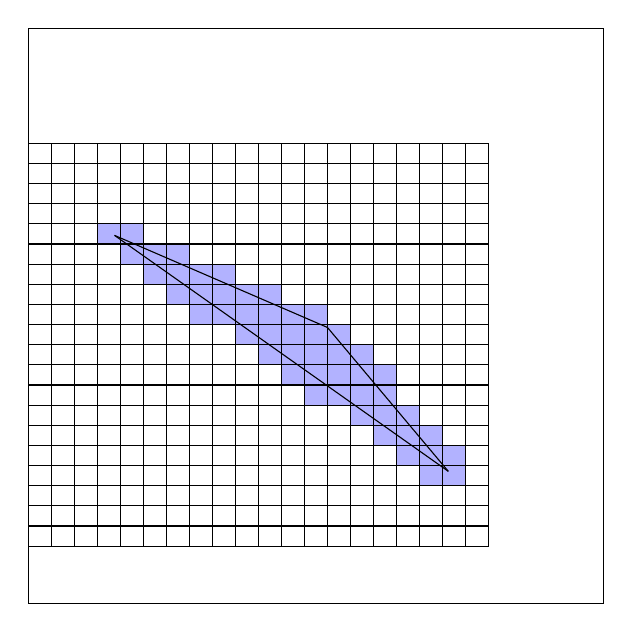
\begin{tikzpicture}
\begin{axis}[clip=false,ticks=none,xmin=0,xmax=\xmax,ymin=0,ymax=\ymax,scale mode=scale uniformly,width=3.5in, height=3.5in]

%% Begin Content

\fill [blue!30!white] (1.2,6.25) rectangle (1.6,6.6);
\fill [blue!30!white] (5.2,4.5) rectangle (5.6,4.85);
\fill [blue!30!white] (7.2,2.05) rectangle (7.6,2.4);
\fill [blue!30!white] (1.2,6.25) rectangle (1.6,6.6);
\fill [blue!30!white] (1.6,5.9) rectangle (2,6.25);
\fill [blue!30!white] (1.6,6.25) rectangle (2,6.6);
\fill [blue!30!white] (2,5.55) rectangle (2.4,5.9);
\fill [blue!30!white] (2,5.9) rectangle (2.4,6.25);
\fill [blue!30!white] (2.4,5.2) rectangle (2.8,5.55);
\fill [blue!30!white] (2.4,5.55) rectangle (2.8,5.9);
\fill [blue!30!white] (2.4,5.9) rectangle (2.8,6.25);
\fill [blue!30!white] (2.8,4.85) rectangle (3.2,5.2);
\fill [blue!30!white] (2.8,5.2) rectangle (3.2,5.55);
\fill [blue!30!white] (2.8,5.55) rectangle (3.2,5.9);
\fill [blue!30!white] (3.2,4.85) rectangle (3.6,5.2);
\fill [blue!30!white] (3.2,5.2) rectangle (3.6,5.55);
\fill [blue!30!white] (3.2,5.55) rectangle (3.6,5.9);
\fill [blue!30!white] (3.6,4.5) rectangle (4,4.85);
\fill [blue!30!white] (3.6,4.85) rectangle (4,5.2);
\fill [blue!30!white] (3.6,5.2) rectangle (4,5.55);
\fill [blue!30!white] (4,4.15) rectangle (4.4,4.5);
\fill [blue!30!white] (4,4.5) rectangle (4.4,4.85);
\fill [blue!30!white] (4,4.85) rectangle (4.4,5.2);
\fill [blue!30!white] (4,5.2) rectangle (4.4,5.55);
\fill [blue!30!white] (4.4,3.8) rectangle (4.8,4.15);
\fill [blue!30!white] (4.4,4.15) rectangle (4.8,4.5);
\fill [blue!30!white] (4.4,4.5) rectangle (4.8,4.85);
\fill [blue!30!white] (4.4,4.85) rectangle (4.8,5.2);
\fill [blue!30!white] (4.8,3.45) rectangle (5.2,3.8);
\fill [blue!30!white] (4.8,3.8) rectangle (5.2,4.15);
\fill [blue!30!white] (4.8,4.15) rectangle (5.2,4.5);
\fill [blue!30!white] (4.8,4.5) rectangle (5.2,4.85);
\fill [blue!30!white] (4.8,4.85) rectangle (5.2,5.2);
\fill [blue!30!white] (5.2,3.45) rectangle (5.6,3.8);
\fill [blue!30!white] (5.2,3.8) rectangle (5.6,4.15);
\fill [blue!30!white] (5.2,4.15) rectangle (5.6,4.5);
\fill [blue!30!white] (5.2,4.5) rectangle (5.6,4.85);
\fill [blue!30!white] (5.6,3.1) rectangle (6,3.45);
\fill [blue!30!white] (5.6,3.45) rectangle (6,3.8);
\fill [blue!30!white] (5.6,3.8) rectangle (6,4.15);
\fill [blue!30!white] (5.6,4.15) rectangle (6,4.5);
\fill [blue!30!white] (6,2.75) rectangle (6.4,3.1);
\fill [blue!30!white] (6,3.1) rectangle (6.4,3.45);
\fill [blue!30!white] (6,3.45) rectangle (6.4,3.8);
\fill [blue!30!white] (6,3.8) rectangle (6.4,4.15);
\fill [blue!30!white] (6.4,2.4) rectangle (6.8,2.75);
\fill [blue!30!white] (6.4,2.75) rectangle (6.8,3.1);
\fill [blue!30!white] (6.4,3.1) rectangle (6.8,3.45);
\fill [blue!30!white] (6.8,2.05) rectangle (7.2,2.4);
\fill [blue!30!white] (6.8,2.4) rectangle (7.2,2.75);
\fill [blue!30!white] (6.8,2.75) rectangle (7.2,3.1);
\fill [blue!30!white] (7.2,2.05) rectangle (7.6,2.4);
\fill [blue!30!white] (7.2,2.4) rectangle (7.6,2.75);
\draw[black] (0,1) -- (0,8);
\draw[black] (0,1) -- (8,1);
\draw[black] (0.4,1) -- (0.4,8);
\draw[black] (0,1.35) -- (8,1.35);
\draw[black] (0.8,1) -- (0.8,8);
\draw[black] (0,1.7) -- (8,1.7);
\draw[black] (1.2,1) -- (1.2,8);
\draw[black] (0,2.05) -- (8,2.05);
\draw[black] (1.6,1) -- (1.6,8);
\draw[black] (0,2.4) -- (8,2.4);
\draw[black] (2,1) -- (2,8);
\draw[black] (0,2.75) -- (8,2.75);
\draw[black] (2.4,1) -- (2.4,8);
\draw[black] (0,3.1) -- (8,3.1);
\draw[black] (2.8,1) -- (2.8,8);
\draw[black] (0,3.45) -- (8,3.45);
\draw[black] (3.2,1) -- (3.2,8);
\draw[black] (0,3.8) -- (8,3.8);
\draw[black] (3.6,1) -- (3.6,8);
\draw[black] (0,4.15) -- (8,4.15);
\draw[black] (4,1) -- (4,8);
\draw[black] (0,4.5) -- (8,4.5);
\draw[black] (4.4,1) -- (4.4,8);
\draw[black] (0,4.85) -- (8,4.85);
\draw[black] (4.8,1) -- (4.8,8);
\draw[black] (0,5.2) -- (8,5.2);
\draw[black] (5.2,1) -- (5.2,8);
\draw[black] (0,5.55) -- (8,5.55);
\draw[black] (5.6,1) -- (5.6,8);
\draw[black] (0,5.9) -- (8,5.9);
\draw[black] (6,1) -- (6,8);
\draw[black] (0,6.25) -- (8,6.25);
\draw[black] (6.4,1) -- (6.4,8);
\draw[black] (0,6.6) -- (8,6.6);
\draw[black] (6.8,1) -- (6.8,8);
\draw[black] (0,6.95) -- (8,6.95);
\draw[black] (7.2,1) -- (7.2,8);
\draw[black] (0,7.3) -- (8,7.3);
\draw[black] (7.6,1) -- (7.6,8);
\draw[black] (0,7.65) -- (8,7.65);
\draw[black] (8,1) -- (8,8);
\draw[black] (0,8) -- (8,8);
\draw[black] (1.5,6.4) -- (5.2,4.8);
\draw[black] (5.2,4.8) -- (7.3,2.3);
\draw[black] (7.3,2.3) -- (1.5,6.4);

%% End Content

\end{axis}
\end{tikzpicture}
\end{document}
